\documentclass[12pt]{article}
\usepackage[utf8]{inputenc}
\usepackage[russian]{babel}
\usepackage [left=30 mm, top=30 mm, right=30 mm, bottom=20mm, nohead, footskip=10 mm] {geometry}
%\usepackage{pscyr}
\usepackage{multicol}
\usepackage{lipsum}
\usepackage{mwe}
\usepackage[T2A]{fontenc}
\usepackage{amsmath}
\usepackage{amssymb}
\usepackage{graphicx}
\graphicspath{{src/}}
\usepackage{listings}   
\usepackage{hyperref}
\usepackage{fancyhdr}
%\usepackage{algorithm}
\usepackage{algpseudocode}
\usepackage{indentfirst}
\usepackage{listings}
\usepackage{caption}
\usepackage{hyperref}
\addto\captionsrussian{\def\refname{Список источников}}
\hypersetup{
    colorlinks=true,
    linkcolor=blue,
    filecolor=magenta,      
    urlcolor=cyan,
}
\usepackage{float}%"Плавающие" картинки
\hypersetup{
    colorlinks=true,
    linkcolor=blue,
    filecolor=magenta,      
    urlcolor=cyan,
    pdftitle={Sharelatex Example},
    bookmarks=true,
    pdfpagemode=FullScreen,
}
\usepackage{wrapfig}%Обтекание фигур (таблиц, картинок и прочего)

\parindent=24pt


\begin{document}

\begin{center}
\hfill \break
\large{МИНОБРНАУКИ РОССИИ} \\
\hfill \break
\small {ФЕДЕРАЛЬНОЕ ГОСУДАРСТВЕННОЕ БЮДЖЕТНОЕ ОБРАЗОВАТЕЛЬНОЕ УЧРЕЖДЕНИЕ }\\
\small { ВЫСШЕГО ПРОФЕССИОНАЛЬНОГО ОБРАЗОВАНИЯ  } \\
\hfill \break
\normalsize {\textbf{ <<САНКТ-ПЕТЕРБУРГСКИЙ ПОЛИТЕХНИЧЕСКИЙ УНИВЕРСИТЕТ } }\\
{\normalsize {\textbf { ПЕТРА ВЕЛИКОГО>>}}} \\
\hfill \break
\large{Институт Компьютерных Наук и Кибербезопасности }\\
\hfill \break
\large{ Высшая школа технологий искуственного интелекта }\\
\hfill \break
Направление 02.03.01 Математика и Компьютерные Науки\\
\vskip 1cm
\large {Отчет по лабораторной работе №2.}
\vskip 0.2cm
\large {По дисциплине:}

\large{<<Методы тестирования программного обеспечения>>} \\
\hfill \break
\normalsize{Тема Работы:} \\
\hfill \break
\normalsize{<<Тестирование методами "белого" и "черного" ящиков>>} \\
\thispagestyle {empty}

\hfill \break
\vskip 0.3cm
\vskip 1cm
\end{center}
\begin {tabular}{cccc}
\hspace{0.5cm}Обучающийся: &\underline {\hspace{3cm}} &  &Черепанов Михаил Дмитриевич\\\\
\hspace{0.5cm}Руководитель: &\underline {\hspace{3cm}} & &Курочкин Михаил Александрович\\\\
\end{tabular}
\vskip 0.5 cm
\hspace{9cm}\def \hrf#1{\hbox to#1{\hrulefill}}<<\hrf{2em}>>  \hrf{6em}  20\hrf{1em}~r.
\vskip 2cm
\begin {center} Санкт-Петербург 2024 \end{center}
\newpage
\tableofcontents
\newpage






\section*{Введение}
 \addcontentsline{toc}{section}{Введение}
Тестирование является важным этапом разработки программного обеспечения, направленным на обеспечение его качества и надежности. Целью тестирования является выявление ошибок и дефектов в программном продукте до его выпуска в эксплуатацию.

Существует два основных подхода к тестированию программного обеспечения: методом <<Белого ящика>>  и методом <<Черного ящика>>.

Тестирование <<белым>> ящиком основано на анализе внутренней структуры программного кода. При использовании этого подхода тестировщик имеет доступ к исходному коду программы и может осуществлять тестирование на уровне отдельных модулей, функций и логики программы. 

Тестирование <<черным>> ящиком, напротив, основано на внешнем поведении программного продукта без знания его внутренней структуры. При использовании этого подхода тестировщик рассматривает программу как <<черный ящик>>, не обращая внимания на детали реализации. Основная задача тестирования методом <<черного ящика>> - выявить случаи, в которых программа не соответсвует спецификации.


Цель данной лабораторной работы - изучить обе методолгии и  получить практический опыт по их применению.
\newpage

\section{Постановка задачи}

1. Изучить методологии тестирования <<белым>> и  <<черным>> ящиками.

2. Разработать тесты и провести тестирование в соответсвии с каждой из этих методологий для двух предоставленных программ.

\newpage


\section{Общие сведения о тестировании методами <<Белого>>  и <<Черного>> ящиков}

\subsection{Метод <<Черного ящика>>}


Одной из важнейших стратегий тестирования является тестирование методом черного ящика. В соответствии с этим методом программа рассматривается как “черный ящик”, внутреннее поведение и структура которого не имеют никакого значения. Вместо этого все внимание фокусируется на выяснении обстоятельств, при которых поведение программы не соответствует спецификации.


При таком подходе тестовые данные выбираются исключительно на основе требований спецификации (без привлечения каких-либо знаний о внутренней структуре программы).

Обнаружить все ошибки в программе при помощи данного метода
можно было бы выполнив исчерпывающее входное тестирование. Однако в реальных задачах такое тестирование произвести невозможна ввиду
большого (или бесконечного) пространства входных данных. В рамках
рассматриваемого метода существует ряд эвристических методологий,
направленных на то, чтобы минимальным количеством тестов обнаружить как можно большее число ошибок.

  
Далее рассматриваются основные методологии проектирования тестов, используемые в рамках метода "черного ящика".



\subsubsection{Разбиение на классы эквивалентности}

Ис­черпывающее тестирование программы на входных наборах данных
принципиально неосуществимо. Следовательно, тестировщик всегда будет ограничиваться небольшим подмножеством всех возможных входных зна­чений. А раз так, то хотелось бы выбрать “самое подходящее” подмножество тестов, т.е. такое, которое обеспечит наибольшую веро­ятность обнаружения большинства ошибок.

Определить такое “самое подходящее” подмножество можно используя разбиение входных данных программы на конечное число классов эквивалентности.

Это позволит с достаточной долей уверенности  полагать, что тестирование одного конкретного значения из данного класса эквивалентно тестированию любого другого значения, принадлежащего тому же классу.

{\bf Определение классов эквивалентности}

Определение классов эквивалентности сводится к последовательному рассмотрению каждого из входных условий (обычно это предложение или фраза, приведенные в спецификации) и разбиению его на две или несколько групп. Часто на основе спецификации выделяются два типа классов:

1. Допустимые классы эквивалентности, представляющие допустимые входные данные программы.
2. Недопустимые классы эквивалентности, представляющие все остальные возможные со­стояния условий (т.е. недопустимые входные значения).	



\subsubsection{Анализ граничных значений}

Как показывает опыт, тесты, исследующие граничные условия, приносят большую пользу, чем тесты, которые не обеспечивают этого. Граничные условия — это ситуации, возникающие в области гранич­ных значений входных и выходных классов эквивалентности. Анализ гра­ничных значений отличается от методики разбиения на классы эквивалент­ности в двух отношениях.

1. Вместо того чтобы выбирать любой элемент класса эквивалентности в качестве представителя всего класса, анализ граничных значений тре­бует выбирать такой элемент или элементы, которые обеспечивают те­стирование каждой границы класса.

2. При создании тестов внимание фокусируется не только на входных условиях (пространство входных значений), но и на пространстве результатов (выходные классы эквивалентности).


\subsubsection{Применение причинно-следственных диаграмм}

Одной из слабых сторон анализа граничных значений и разбиения дан­ных на классы эквивалентности является то, что они не исследуют комби­наций входных условий.

Тестирование комбинаций входных условий — непростая задача, посколь­ку даже после разбиения входных условий на классы количество возможных комбинаций обычно выражается астрономическими цифрами. В отсутствие систематического способа выбора подмножества входных условий его, как правило, выбирают произвольным образом, что и становится причиной не­эффективного тестирования.




Метод причинно-следственных диаграмм   помогает систематически выбирать высокорезультативные тесты. Его дополнительным преимуществом является то, что он позволя­ет обнаруживать неполноту и неоднозначность исходных спецификаций.

Причинно-следственная диаграмма представляет собой формальный язык, на который транслируется спецификация, написанная на естествен­ном языке. Фактически такая диаграмма является аналогом цифровой логи­ческой схемы, но для ее описания используется более простая нотация по
сравнению с той, которая принята в электронике. Для того чтобы восполь­зоваться методом причинно-следственных диаграмм, никаких знаний элек­троники, кроме понимания правил булевой алгебры (т.е. умения работать с логическими операторами and, or и not), не требуется.


\subsubsection{Стратегия разработки тестов в рамках методики <<Черного ящика>>}

 Каждый метод из перечисленных выше обеспечивает создание определен­ного набора полезных тестов, но ни один из них сам по себе не может обеспечить полный набор тестов. 
 
 Поэтому в рамках тестирования <<Черного ящика>> рекомендуется использовать следующую стратегию:
 
 \begin{enumerate}
 \item Если спецификация содержит комбинации входных условий, то начинать следует с применения метода причинно-следственных диаграмм.
 
 \item В любом случае необходимо использовать анализ граничных значе­ний. Этот метод включает анализ как входных, так и выходных данных. Анализ граничных значений дает набор дополни­тельных тестовых условий, но многие из них могут быть включены в тесты метода причинно-следственных диаграмм.
 
 \item Определить допустимые и недопустимые классы эквивалентности для входных и выходных данных и в случае необходимости создать новые тесты в дополнение к уже имеющимся.
 
 \item Для получения дополнительных тестов рекомендуется использовать метод прогнозирования ошибок. Метод состоит в выдвижении
предположений об ошибках, а также определении тестов, связанных с допущениями, которые программист мог сделать при чтении
спецификации (те моменты, которые не были включены в спецификацию либо случайно, либо из-за того, что автору спецификации
они показались очевидными).
 
     
 \end{enumerate}



\subsection{Метод <<Белого ящика>>}

Тестирование "белым" ящиком основано на анализе внутренней структуры программного кода. При использовании этого подхода тестировщик имеет доступ к исходному коду программы и может осуществлять тестирование на уровне отдельных модулей, функций и логики программы. 

При тестировании методом “белого ящика” учитывается степень покрытия логики (кода) программы. Исчерпывающее тестирование методом “белого ящика” требует прохождения каждого пути в программе,
однако в случае программ, содержащих циклы, удовлетворение этого
условия — задача нереальная. Поэтому существуют различные эвристические правила, позволяющие определить набор критериев, достаточных
для приемлемого тестирования данным методом.

Эти критерии можно упорядочить по возрастанию качества покрытия логики программы следующим образом:


\begin{itemize}
\item Критерий покрытия операторов. В соответствии с данным критерием набор тестов является достаточным, если каждая инструкция
в программе выполняется хотя бы один раз.

\item Критерий покрытия условий. В соответствии с этим критерием
количество тестов должно быть таким, чтобы каждое условие в
программе хотя бы раз принимало как значение true (истина), так
и false (ложь). Также каждая точка входа в програму или
подпрограмму были пройдены хотя бы один раз.



\item Комбинаторное покрытие условий. Этот критерий требует создания такого количества тестов, при котором каждая возможная комбинация результатов вычисления условий в каждом ветвлении и каждая точка входа проверяются по крайней мере один раз.


\end{itemize}










\section{<<Треугольник Паскаля>>}





\subsection{Постановка задачи, спецификация}

{\bf Название:}

Печать N сток треугольника Паскаля

{\bf Дано:}

Число N.

{\bf Требуется:}

Вывести на экран N строк треугольника Паскаля или сообщение об ошибке.

{\bf Ограничение:}

$ 0<=N<=100 $

N - целое число

{\bf Спецификация:}

\vskip 1cm
{
    \centering
    \includegraphics[width=1\linewidth]{spec1.png}
   
    \label{fig:i1}
}
\vskip 1cm


{\bf Блок-схема алгоритма:}

\vskip 1cm
{
    \centering
    \includegraphics[width=0.6\linewidth]{бс1.png}
   
    \label{fig:i1}
}
\vskip 1cm


\vskip 1cm
{
    \centering
    \includegraphics[width=0.7\linewidth]{бс2.png}
   
    \label{fig:i1}
}
\vskip 1cm


\subsection{Составление тестов методом <<черного ящика>>}

{\bf Классы эквивалентности}

Исходя из ограничений для программы составим следующие классы эквивалентности:

\vskip 1cm
{
    \centering
    \includegraphics[width=1\linewidth]{кэ1.png}
   
    \label{fig:i1}
}
\vskip 1cm


Составим тесты для допустимых классов эквивалентности \{1,3\}. Нет оснований предполагать, что некоторые значения из данных классов эквивалентности будут обрабатываться по-разному, поэтому выберем случайные значения:

\vskip 1cm
{
    \centering
    \includegraphics[width=0.7\linewidth]{кэд.png}
   
    \label{fig:i1}
}
\vskip 1cm



В выбранных случаях программа отработала корректно.


Составим тесты для недопустимых классов:

\vskip 1cm
{
    \centering
    \includegraphics[width=1\linewidth]{нкэ.png}
   
    \label{fig:i1}
}
\vskip 1cm



{\bf Проверка граничных условий:}

В спецификации указано единственное условие:

$0<=N<=100$

Для каждой из границ напишем по 5 тестов: граница, наиболее близкое к границе целое число(с низу и сверху), наиболее близкое к границе дробное число(с низу и сверху).


\vskip 1cm
{
    \centering
    \includegraphics[width=1\linewidth]{грусл11.png}
   
    \label{fig:i1}
}
{
    \centering
    \includegraphics[width=0.99\linewidth]{грусл12.png}
   
    \label{fig:i1}
}
\vskip 1cm


{\bf Причинно-следственная диаграмма:}

Для построения причинно-следственной диаграммы еще раз внимательно прочитаем спецификацию и выделим из нее отдельно три причины:

1:   n>=0;

2:   n<100;

3:   n- целое число;


Выделим два следсвия:

11: На экран выводится N строк треугольника Паскаля.

12: На экран выводится сообщение об ошибке.

Построим причинно-следственную диаграмму:

\vskip 1cm
{
    \centering
    \includegraphics[width=0.5\linewidth]{псд1.png}
   
    \label{fig:i1}
}
\vskip 1cm

В соответствии с методолгоией причинно следственных диаграмм необходимо для единственного желаемого условия рассмотреть все комбинации порождающих его условий.

Таким образом, требуется разработать один тест, проверяющий выполнимость одновременно 1,2 и 3 условий.

\vskip 1cm
{
    \centering
    \includegraphics[width=1\linewidth]{одинтест1.png}
   
    \label{fig:i1}
}
\vskip 1cm


\subsection{Составление тестов методом <<белого ящика>>}
Алгоритм составления тестов методом белого ящика предполагает обход всех возможных путей в теле программы и проверка выполнения каждого оператора не менее одного раза.

Для этого обозначим каждый из блоков условий, и блоки, находящиеся в разных ветках программы отдельным символом.



\vskip 1cm
{
    \centering
    \includegraphics[width=0.5\linewidth]{диаг11.png}
   
    \label{fig:i1}
}
\vskip 1cm

\vskip 1cm
{
    \centering
    \includegraphics[width=0.8\linewidth]{диаг12.png}
   
    \label{fig:i1}
}
\vskip 1cm




Выделим следующие пути в теле программы, которые необходимо покрыть тестами:

ABC

ABDE

ABDFG

ABDFHIJ

ABDFHIKNPM

ABDFHIKNOPM

Другие пути во время исполнения программы невозможны.

Каждый из выделенных путей покроем тестами:

ABC:  строка ":q"

ABDE:   1.5 (Любое значение, не являющееся целым числом)

ABDFG:    -1 (Любое отрицательное число)

ABDFHIJ:   0

ABDFHIKNPMJ: 4 (Любое целое число$\in [1,100]$)

ABDFHIKNOPMJ:  4 (Любое целое число$\in [1,100]$)

Входные данные для двух последних выделенных путей совпадают, так как в любом случае при прохождении одного из них, программа зайдет во второй.



Итак, в в ходе тестирования методом <<белого ящика>> были разработаны следующие тесты:


\vskip 1cm
{
    \centering
    \includegraphics[width=0.8\linewidth]{tablewb1.png}
   
    \label{fig:i1}
}
\vskip 1cm

\subsection{Тестирование}


Таким образом, пользуясь методами <<Черного>> и <<Белого>>
ящиков, можно составить следующий набор тестов, покрывающий граничные условия, все выделенные классы эквивалентности, все пути в теле программы.

\vskip 1cm
{
    \centering
    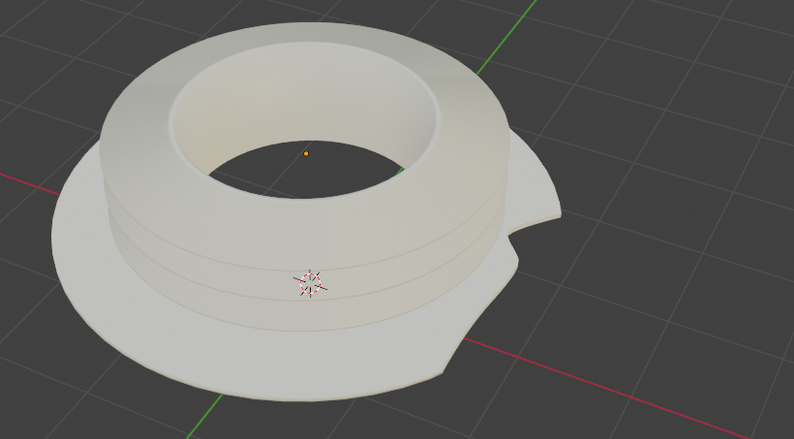
\includegraphics[width=1\linewidth]{final1.png}
   
    \label{fig:i1}
}



В ходе тестирования программы несоответсвий спецификации и ошибок в логике программы обнаружено не было.






\newpage


\section{<<Проверка правильности скобочной последовательности>>}


\subsection{Постановка задачи, спецификация}

{\bf Название:}

Проверка правильности скобочной последовательности.

{\bf Дано:}

Строка, в которой могут содержаться скобочные символы:

  << \{, \} , [ , ] , ( , )>>, а так же другие символы.

{\bf Требуется:}

Проверить правильность скобочных последовательностей внутри строки.

Проверяются скобочные последовательности трех типов: 

состоящие из круглых скобок: ();

состоящие из фигурных скобок: \{\};

состоящие из квадратных скобок: [];


В случае, если каждый из трех типов последовательностей верен - вывести на экран <<Да>>.

Иначе - <<Нет>>.

В случае, если размер строки превышает 10000 символов - вывести сообщение об ошибке.


{\bf Ограничение:}

Длина строки не более 10000 символов.


{\bf Спецификация:}

\vskip 1cm
{
    \centering
    \includegraphics[width=1\linewidth]{spec2.png}
   
    \label{fig:i1}
}
\vskip 1cm

{\bf Блок-схема алгоритма:}

\vskip 1cm
{
    \centering
    \includegraphics[width=0.6\linewidth]{бс21.png}
   
    \label{fig:i1}
}
\vskip 1cm


\vskip 1cm
{
    \centering
    \includegraphics[width=0.7\linewidth]{бс22.png}
   
    \label{fig:i1}
}
\vskip 1cm






\subsection{Составление тестов методом <<черного ящика>>}

{\bf Классы эквивалентности}

Исходя из спецификации составим следующие классы эквивалентности:

\vskip 1cm
{
    \centering
    \includegraphics[width=1\linewidth]{2кэ.png}
   
    \label{fig:i1}
}
\vskip 1cm


Составим тесты для допустимых классов эквивалентности \{1,3,5,7\}. Нет оснований предполагать, что некоторые значения из данных классов эквивалентности будут обрабатываться по-разному, поэтому выберем случайные значения для каждого из допустимых классов:

\vskip 1cm
{
    \centering
    \includegraphics[width=1\linewidth]{2дкэ.png}
   
    \label{fig:i1}
}
\vskip 1cm


Составим тесты для недопустимых классов:

\vskip 1cm
{
    \centering
    \includegraphics[width=1\linewidth]{ндкэ.png}
   
    \label{fig:i1}
}
\vskip 1cm


{\bf Проверка граничных условий}


В спецификации указано единственное граничное условие:

Длина строки < 10 000 символов.
Т.к. длина не может быть отрицательным числом, граничным условием так же является пустая строка(длины 0).

Поэтому проверим верхнюю границу, наиболее близкое к ней значение сверху и снизу, нижнюю границу, наиболее близкое к ней верхнее значение:

\vskip 1cm
{
    \centering
    \includegraphics[width=1\linewidth]{2грусл.png}
   
    \label{fig:i1}
}
\vskip 1cm


{\bf Причинно-следственная диаграмма:}

Для составления диаграммы выделим следующие причины из спецификации:

1. Корректная расстановка в строке символов:  <<(>> или <<)>>;

2. Корректная расстановка в строке символов:  <<\{>> или <<\}>>;

3. Корректная расстановка в строке символов:  <<[>> или <<]>>;

4. Длина строки $<= 10 000$ символов;

Были выделены следующие следствия:

11.  Вывод <<Да>>  при корректности скобочной последовательности.

12.  Вывод <<Нет>>  при некорректности скобочной последовательности.

13.  Вывод сообщения об ошибке  при длинне строки превышающей 10 000.

Построим причинно следственную диаграмму:




\vskip 1cm
{
    \centering
    \includegraphics[width=0.6\linewidth]{2прслд.png}
   
    \label{fig:i1}
}
\vskip 1cm


Применим метод обратной трассировки графа, который заключается в обходе диаграммы от следствий к условиям:

Указания к методу обратной трассировки графа:

1. Если путь обратной трассировки проходит через узел типа or, выход которого должен принимать значение 1, то не следует одновременно устанавливать в 1 более одного входа в этот узел.

2. Если путь обратной трассировки проходит через узел типа and, вы­ход которого должен принимать значение 0, то, конечно же, должны быть перечислены все комбинации входов, приводящие к установке выхода в 0. 

3. Если путь обратной трассировки проходит через узел типа and, выход которого должен принимать значение 0, то необходимо указать лишь одно условие, при котором все входы являются нулями.

Исходя из вышеперечисленных правил построим тесты, проверяющие условия 1,2,3,4 -  поотдельности друг от друга;

Выполнение условий 1,2,3,4 - одновременно.

Данные тесты покрывающие данные условия уже были сгенерированны в предыдущих пунктах.

Так как в данном случае строка, не содержащая скобок интерперетируется как правильная скобочная последовательность, и есть основания предполагать, что строка в которой присутствуют скобки обрабатывается отлично от пустой строки - добавим следующий тест:




\vskip 1cm
{
    \centering
    \includegraphics[width=1\linewidth]{2одинтест.png}
   
    \label{fig:i1}
}
\vskip 1cm


\subsection{Составление тестов методом <<белого ящика>>}


Для составления тестов обозначим каждый из блоков условий и блоки, находящиеся в разных ветках программы отдельными символами на блок-схеме:


\vskip 1cm
{
    \centering
    \includegraphics[width=0.6\linewidth]{2бс1.png}
   
    \label{fig:i1}
}
\vskip 1cm
\vskip 1cm
{
    \centering
    \includegraphics[width=0.6\linewidth]{2бс2.png}
   
    \label{fig:i1}
}
\vskip 1cm

После исследования блок-схемы были выделены следующие маршруты:

$
ABC 
$

$
ABDE
$

$
ABDA_1B_1C_1G_1FG
$

$
ABDA_1B_1D_1E_1F_1FH
$

$
ABDA_1B_1D_1E_1C_1G_1H_1FG
$

$
ABDA_1B_1D_1E_1C_1G_1F_1FH
$

Другие маршруты во время выполнения программы невозможны.

\vskip 1cm

Каждый из выделенных маршрутов покроем тестами:



$
ABC 
$  -- <<:q>>

$
ABDE
$ -- <<.....>>(длина строки >10 000)

$
ABDA_1B_1C_1G_1FG
$ -- <<aaa>> (отсутствуют скобки)

$
ABDA_1B_1D_1E_1F_1FH
$ -- <<(aaa]>> (после скобки одного вида, идет скобка другого вида)

$
ABDA_1B_1D_1E_1C_1G_1H_1FG
$  -- <<(aaa)>> (корректная последовательность)

$
ABDA_1B_1D_1E_1C_1G_1F_1FH
$ -- <<(aa>> (после открывающейся скобки отсутсвует закрывающаяся)

В результате анализа был сгенерирован следующий набор тестов:

\vskip 1cm
{
    \centering
    \includegraphics[width=1\linewidth]{2бят.png}
   
    \label{fig:i1}
}


\subsection{Тестирование}


Таким образом, пользуясь методами <<Черного>> и <<Белого>>
ящиков, можно составить следующий набор тестов, покрывающий граничные условия, все выделенные классы эквивалентности, все пути в теле программы.

\vskip 1cm
{
    \centering
    \includegraphics[width=1\linewidth]{2final1.png}
   
    \label{fig:i1}
}


{
    \centering
    \includegraphics[width=1\linewidth]{2final2.png}
   
    \label{fig:i1}
}

\vskip 1cm
В ходе тестирования программы несоответсвий спецификации и ошибок в логике программы обнаружено не было.



\newpage

\section*{Заключение}
 \addcontentsline{toc}{section}{Заключение}
В ходе выполнения работы были изучены стратегии тестирования методами <<белого>> и <<черного>> ящиков и их совместное применение для генерации лучшего покрытия кода тестами.

Были разработаны тесты для двух предоставленных программ, путем последовательного применения стратегий:
 сначала <<черного>> ящика, затем <<белого ящика>>.
 
 В ходе тестирования ошибок в логике программ и несоответсвий спецификации обнаружено не было, но это может сведетельствовать о том, что в данных программах действительно нет ошибок, поскольку предоставленные программы не являются объемными. Тестирование проводилось исключительно в учебных целях. На реальных проектах применные стратегии тестирования должны дать положительные результаты.












 \addcontentsline{toc}{section}{Список использованных источников}
 \newpage
\renewcommand{\refname}{Список использованных источников}
\begin{thebibliography}{99}

  

    \bibitem{source2}  {ИСКУССТВО ТЕСТИРОВАНИЯ ПРОГРАММ.
Третье издание. Гленфорд Майерс, Том Баджетт, Кори Сандлер}
    
     

\end{thebibliography}












\end{document}